%%%% CAPÍTULO 3 - MATERIAL E MÉTODOS (PODE SER OUTRO TÍTULO DE ACORDO COM O TRABALHO REALIZADO)

\chapter{Metodologia}\label{cap:materialemetodos}

O trabalho será dividido em três etapas principais: o desenvolvimento do \textit{software}, 
do \textit{hardware}, e a execução dos testes. Sendo a primeira etapa 
destinada ao desenvolvimento do algoritmo de reconhecimento facial, utilizando os 
recursos da biblioteca OpenCV para o processamento de imagens.

O fluxograma da \autoref{fig:fluxoprog} mostra de maneira simplificada e intuitiva
como o sistema vai tratar as entradas dos sinais (imagens), até validar os resultados.

\begin{figure}[h!]
    \centering
    \caption{Fluxograma do Programa}
    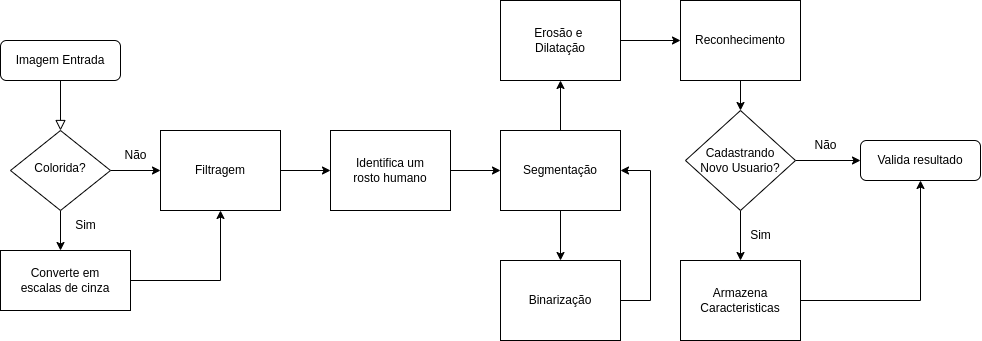
\includegraphics[scale=0.4]{figuras/fluxo_programa.png} 
    \fonte{}%% Fonte
    \label{fig:fluxoprog}
    \centering
\end{figure}

Porém para executar esse algoritmo, será necessário a utilização de um \textit{hardware} 
capaz de processá-lo, desta forma, a segunda etapa será responsável pela montagem 
do protótipo. Onde os \textit{hardwares} que serão utilizados, não são muito complexos, 
sendo compostos por módulos para aquisição dos sinais, processamento e o acionamento 
referente ao controle de acesso.

A terceira e última etapa será referente a validação do protótipo, desde testes, 
ajustes no algoritmo, até melhorias e atualização no hardware. Nessa etapa será 
analisada a assertividade do código desenvolvido e também a sua viabilidade para
utilização no dia-a-dia.

\section{Computador de placa única}\label{sec:materiais}

O \textit{hardware} principal do protótipo, será o ESP32-CAM (\autoref{fig:espcam}) da Espressif®. 
Este dispositivo apesar de ser simples e compacto é ideal para este projeto,  
pois além de possuir uma câmera integrada a sua placa, possui uma capacidade de 
execução em quase tempo real. Sendo este também, o responsável por 
processar, analisar e controlar os demais hardwares. 

\begin{figure}[h!]
    \centering
    \caption{ESP32-CAM}
    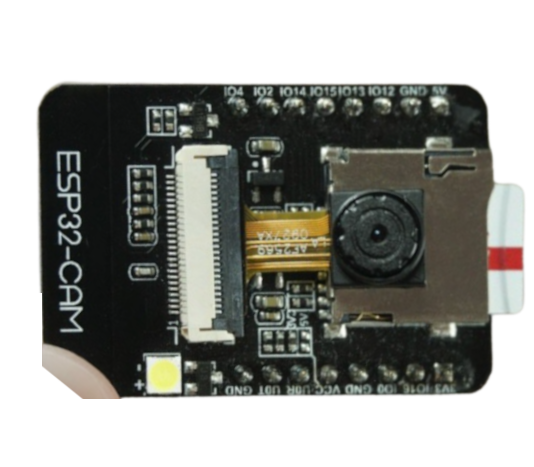
\includegraphics[scale=0.25]{figuras/esp32cam.png} 
    \legend{Fonte: Adaptado de \citeonline{espcamimg}.}
    \label{fig:espcam}
    \centering
\end{figure}

\section{Interface gráfica}\label{sec:materiais}

Para uma melhor interação do usuário com o protótipo, será utilizado o \textit{hardware} 
Nextion Intellignet (\autoref{fig:nextion}), display capaz de fornecer uma interface de controle e visualização 
de forma simples e rápida. Além desses fatores, essa placa possui um editor visual 
com inúmeros componentes e recursos, desta forma, facilitando e reduzindo o tempo 
de programação.

\begin{figure}[h!]
    \centering
    \caption{Nextion Intellignet}
    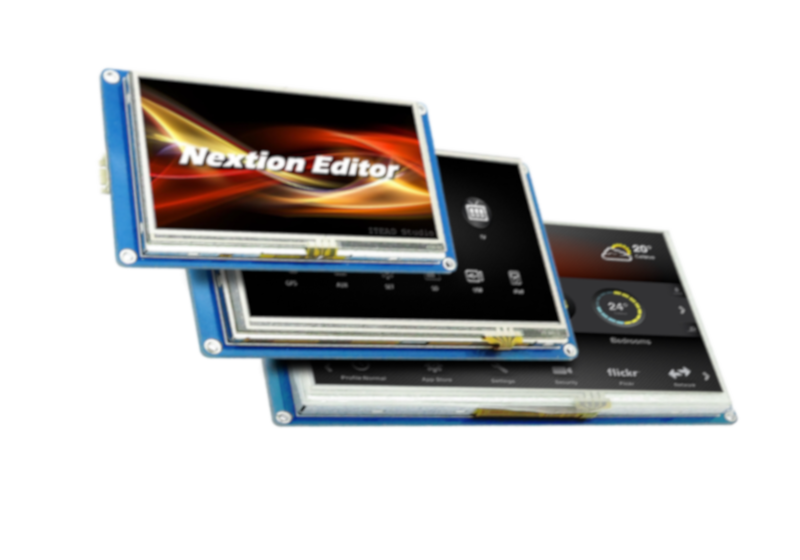
\includegraphics[scale=0.3]{figuras/nextion.png} 
    \legend{Fonte: Adaptado de \citeonline{nextionimg}.}
    \label{fig:nextion}
    \centering
\end{figure}

\section{Fechadura eletrônica}\label{sec:materiais}

O controle de acesso só será funcional se houver uma fechadura eletrônica 
integrada ao seu sistema. Desta forma, o protótipo utilizará o Fecho Elétrico (\autoref{fig:fecho}) 
da AGL. Este que é indicado para portas internas, seja de madeira ou metal, sendo 
acionado por uma tensão em 12v. Desta forma, se o usuário estiver cadastrado e o sistema validar suas credenciais. 
A trava elétrica será acionada e então seu acesso será liberado.


\begin{figure}[h!]
    \centering
    \caption{Fecho Elétrico}
    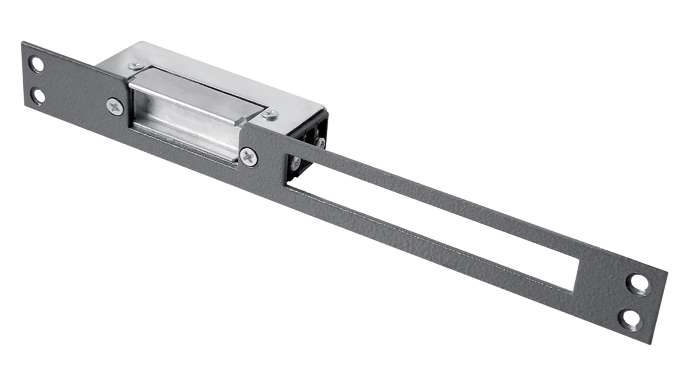
\includegraphics[scale=0.3]{figuras/fechoagl.png} 
    \legend{Fonte: Adaptado de \citeonline{fechaduraimg}.}
    \label{fig:fecho}
    \centering
\end{figure}